%Beamer class
\documentclass{beamer}

\usepackage[czech]{babel}
\usepackage[utf8]{inputenc}
\usepackage{fontenc}
\usepackage{tgheros}
\usepackage{array}
\usepackage{color}
\usepackage{hyperref}

\usetheme{AnnArbor}
\usecolortheme{crane}


\title[Instalace KiCAD]{Instalace KiCAD}
\subtitle[KEO] {Konstrukce a realizace elektronických obvodů}
\author[Brejcha]{\texorpdfstring{Michal Brejcha\newline\url{brejcmic@fel.cvut.cz}}{Michal Brejcha}}
\institute[ČVUT]{ČVUT v Praze, FEL}
\date[Praha, 2025]{Praha, 2025}

%------------------------------------------------------------------------------
%Konstanty a definice
%------------------------------------------------------------------------------
\newtheorem{myDef}{}
\newcommand{\kicadVersion}{9.0.5}

\begin{document}
%------------------------------------------------------------------------------
%Uvodni slajd
%------------------------------------------------------------------------------
\frame{\titlepage}

\begin{frame}
\frametitle{Obsah} 
\tableofcontents
\end{frame}

\AtBeginSection[]
{
  \begin{frame}
    \frametitle{Téma}
    \tableofcontents[currentsection]
  \end{frame}
}

%------------------------------------------------------------------------------
%Instalace KiCAD
%------------------------------------------------------------------------------
\section{\texorpdfstring{Instalace KiCAD}{Instalace Kicad}}
%------------------------------------------------------------------------------
	\begin{frame}
    \frametitle{Stažení návrhového systému KiCAD}
		
		\begin{description}
			\item[url:] \url{http://kicad.org/}
			\item[sekce:] download
		\end{description}
		
		\begin{center}
			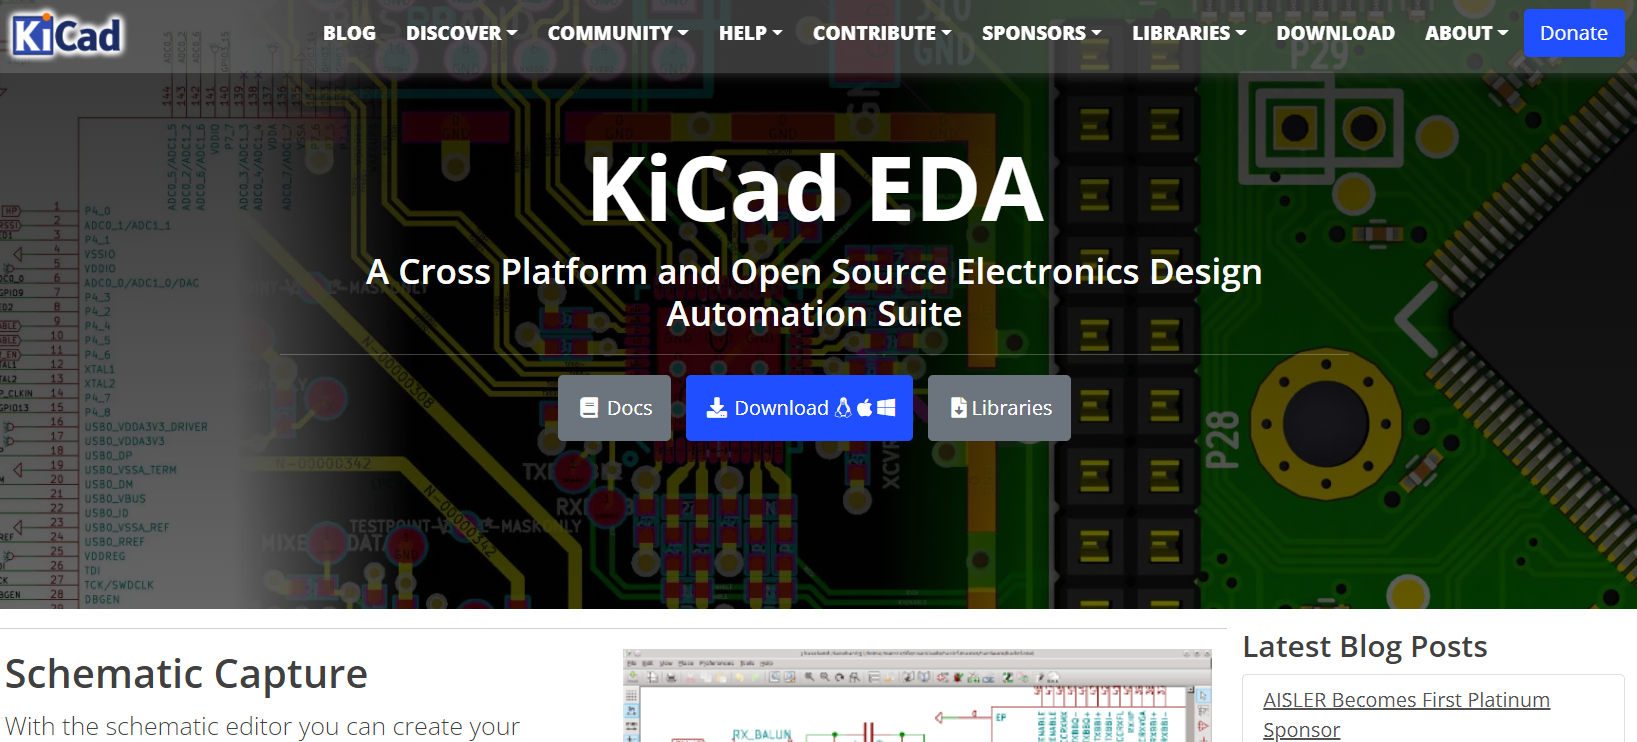
\includegraphics[scale=0.3]{obr/kicad_url.png}
		\end{center}
	\end{frame}
%------------------------------------------------------------------------------
	\begin{frame}
    \frametitle{Výběr operačního systému}
		\small
		\begin{itemize}
			\item instalace windows již obsahuje všechny knihovny
			\item v případě ubuntu je třeba přidat ppa, aby se stáhla poslední verze KiCAD \kicadVersion\
		\end{itemize}
		
		\begin{center}
			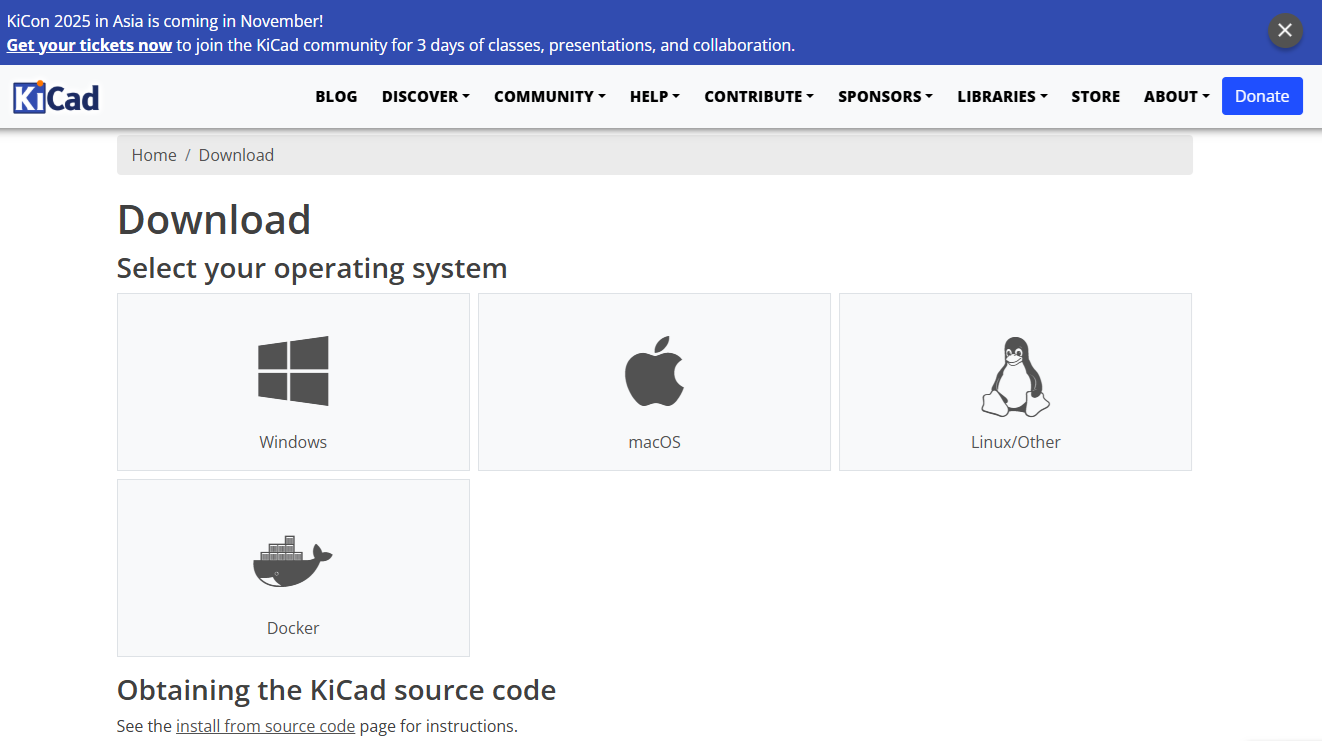
\includegraphics[scale=0.3]{obr/kicad_dwnld.png}
		\end{center}
	\end{frame}
%------------------------------------------------------------------------------
	\begin{frame}
    \frametitle{Stažení instalačního souboru}
		\small
		\begin{itemize}
			\item stáhnout aktuální stabilní verzi \kicadVersion\
		\end{itemize}
		
		\begin{center}
			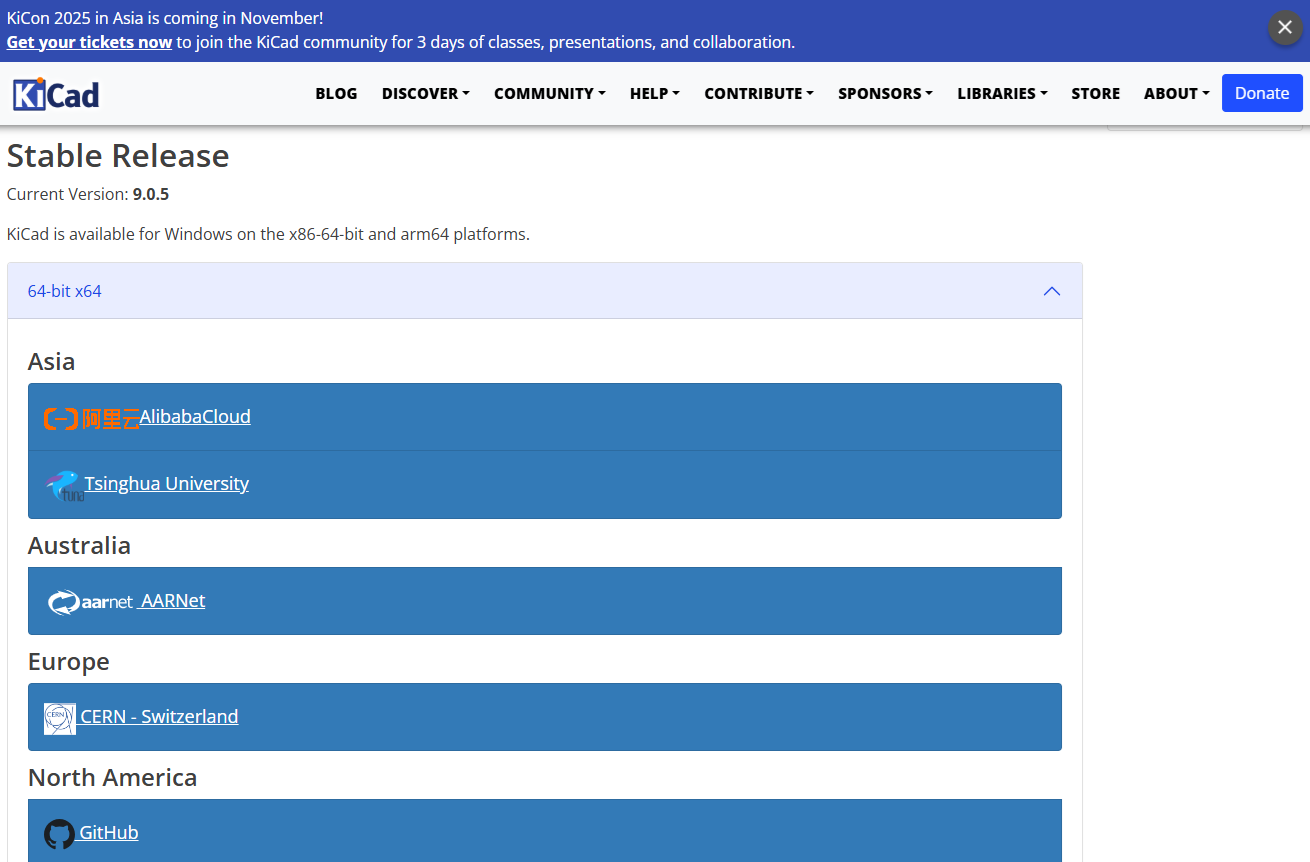
\includegraphics[scale=0.3]{obr/kicad_stbv.png}
		\end{center}
	\end{frame}
%------------------------------------------------------------------------------
	\begin{frame}
    \frametitle{Instalace - Windows}
    	\textbf{Vhodný návod v podobě videa na youtube:} \url{https://www.youtube.com/watch?v=WRple05v3sE} \\~\\
    	
    	\textbf{Shrnutí postupu:}
		\begin{enumerate}
			\item poklepat na stažený instalační soubor
			\item v prvním okně zvolit další,
			\item ponechte volbu instalace všem uživatelům,
			\item vše ve volbě součástí nechat zaškrtnuté, pokud chcete ušetřit místo, vynechte 3D modely,
			\item zvolit další a přejít do nastavení umístění, umístění doporučuji nechat původní předepsané,
			\item zvolit další a nechat proběhnout instalaci
		\end{enumerate}
		
	\end{frame}
%------------------------------------------------------------------------------
	\begin{frame}
    \frametitle{Průběh instalace}
		\begin{center}
			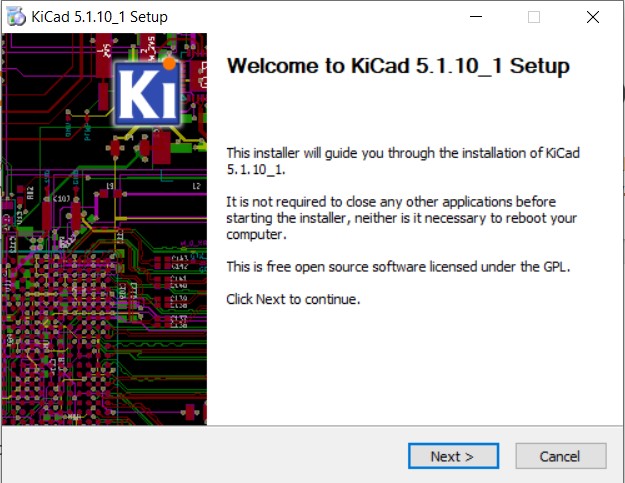
\includegraphics[scale=0.5]{obr/kicad_inst1.png}
		\end{center}
		
		\begin{itemize}
			\item Zde zvolte \uv{Next}.
		\end{itemize}
	\end{frame}
%------------------------------------------------------------------------------
	\begin{frame}
    \frametitle{Průběh instalace}
		\begin{center}
			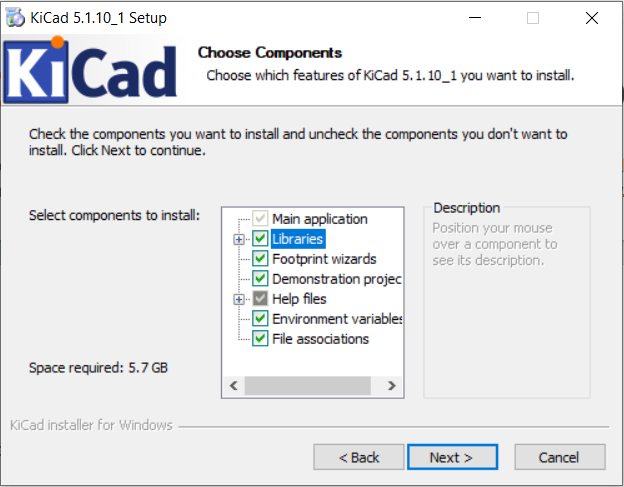
\includegraphics[scale=0.5]{obr/kicad_inst2.png}
		\end{center}
		
		\begin{itemize}
			\item Ponechte volbu pro všechny uživatele počítače.
		\end{itemize}
	\end{frame}
%------------------------------------------------------------------------------
	\begin{frame}
    \frametitle{Průběh instalace}
		\begin{center}
			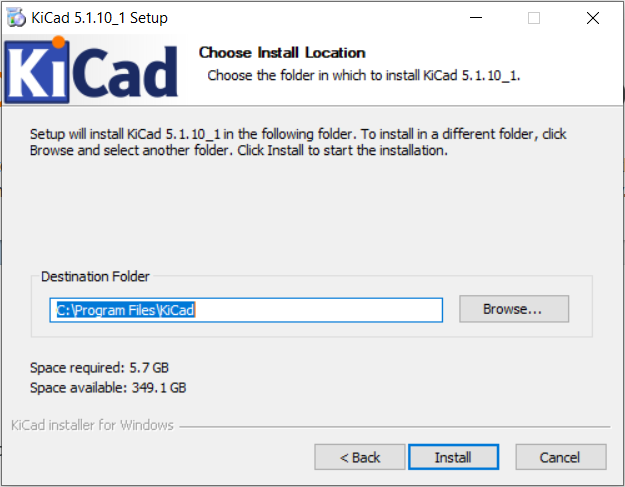
\includegraphics[scale=0.5]{obr/kicad_inst3.png}
			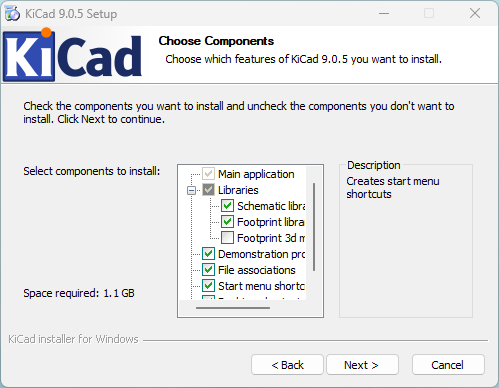
\includegraphics[scale=0.4]{obr/kicad_inst3_no3D.png}
		\end{center}
		
		\begin{itemize}
			\item Vše lze nechat. Zvažte, jestli chcete 3D modely. Rozdíl v nárocích na místo na disku je velký ($>$4 GB).
		\end{itemize}
	\end{frame}
%------------------------------------------------------------------------------
	\begin{frame}
    \frametitle{Průběh instalace}
		\begin{center}
			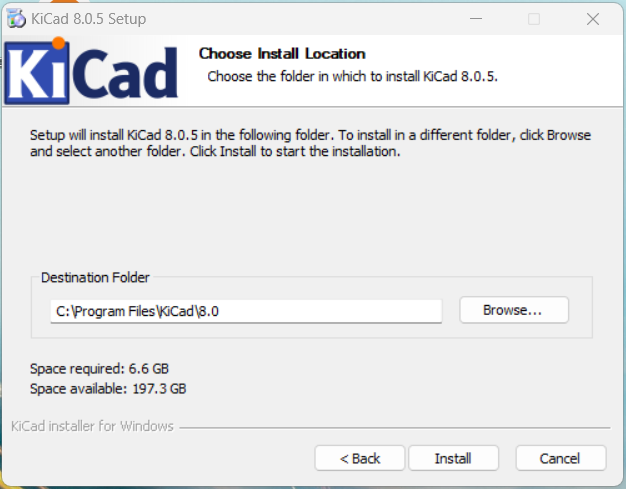
\includegraphics[scale=0.5]{obr/kicad_inst4.png}
		\end{center}
		
		\begin{itemize}
			\item Nechte původní cestu a zvolte \uv{Install}
		\end{itemize}
	\end{frame}
%------------------------------------------------------------------------------
	\begin{frame}
    \frametitle{Průběh instalace}
		\begin{center}
			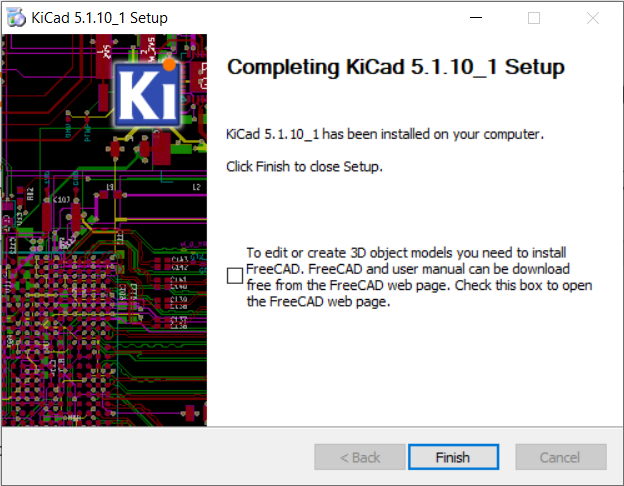
\includegraphics[scale=0.5]{obr/kicad_inst5.png}
		\end{center}
		
		\begin{itemize}
			\item Vyčkejte do konce instalace.
		\end{itemize}
	\end{frame}
%------------------------------------------------------------------------------
	\begin{frame}
    \frametitle{Průběh instalace}
		\begin{center}
			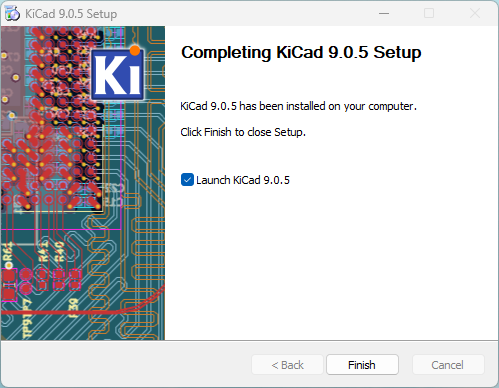
\includegraphics[scale=0.5]{obr/kicad_inst6.png}
		\end{center}
		
		\begin{itemize}
			\item Potvrďte dokončení instalace. Můžete okamžitě přejít na spuštění programu.
		\end{itemize}
	\end{frame}
	
%------------------------------------------------------------------------------
%Instalace KiCAD
%------------------------------------------------------------------------------
\section{\texorpdfstring{První spuštění KiCAD}{Prvni spusteni KiCAD}}
%------------------------------------------------------------------------------
	\begin{frame}
    \frametitle{První spuštění}
    \small
    	Po instalaci se v nabídce start objeví několik nových programů:
      \begin{tabular}{ m{6cm} m{2cm} }
         \begin{itemize}
           \item \textbf{KiCad}
           \item Schematic Editor
           \item PCB Editor
           \item Gerber Viewer
           \item Calculator Tools
           \item Drawing Sheet Editor
					 \item Image Converter
					 \item KiCad Command Prompt
         \end{itemize}
         & 
        \begin{minipage}{\textwidth}
          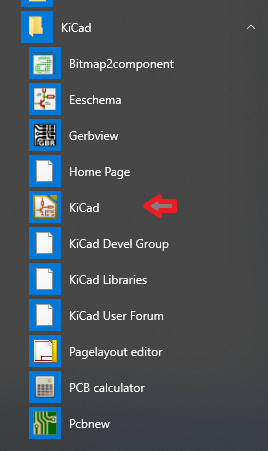
\includegraphics[scale=0.3]{obr/nabStart.png}
        \end{minipage}
				\vspace{0.2cm}
      \end{tabular} 
   
  Vždy spouštíme KiCad, zde se spravují projekty.
	\end{frame}
%------------------------------------------------------------------------------
	\begin{frame}
    \frametitle{První spuštění}
    \small
    V případě, že jste již nějakou instalaci KiCad nainstalovali v minulosti, tak se program dotáže zda má proběhnout import nastavení z předchozí verze. Předpokládejme, že všichni zde zvolíme \uv{výchozí nastavení}.
		
    \begin{center}
			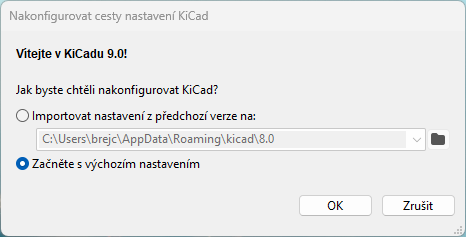
\includegraphics[scale=0.5]{obr/kicad_pocatecni_spusteni.png}
		\end{center}
	\end{frame}
%------------------------------------------------------------------------------
	\begin{frame}
    \frametitle{První spuštění}
    \small
    Následuje dotaz na pomoc se sběrem diagnostických dat pro vývojáře. Zde zvolte podle vlastního úsudku, volba neovlivní chod programu.
		
    \begin{center}
			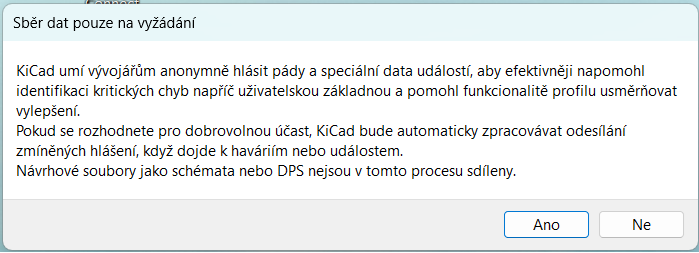
\includegraphics[scale=0.5]{obr/kicad_pocatecni_spusteni2.png}
		\end{center}
	\end{frame}
%------------------------------------------------------------------------------
	\begin{frame}
    \frametitle{První spuštění}
    \small
    Nakonec se dostanete do hlavní nabídky programu, kde se zakládají projekty.
		
    \begin{center}
			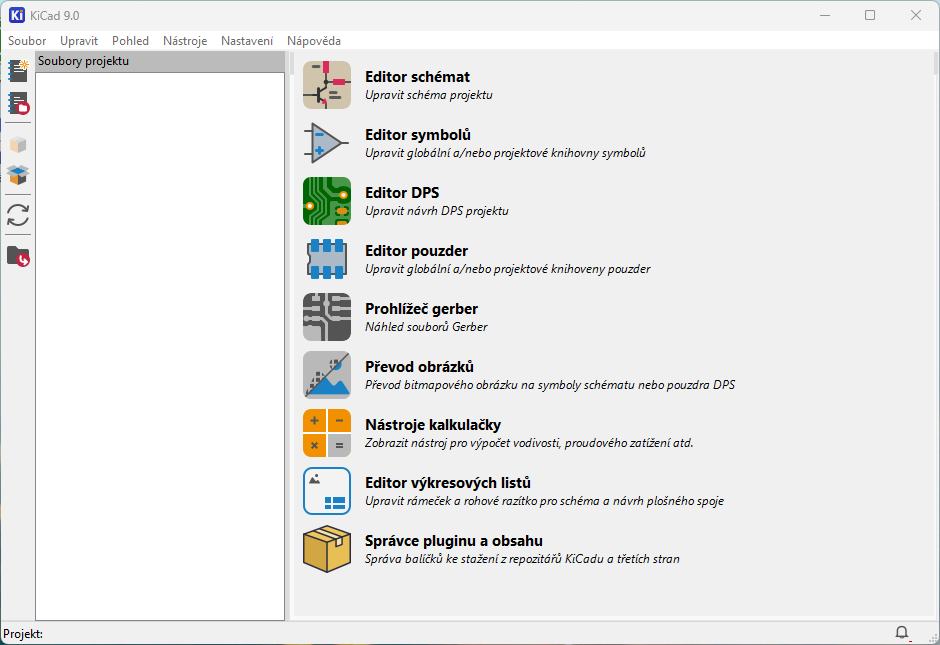
\includegraphics[scale=0.5]{obr/kicad_pocatecni_spusteni3.png}
		\end{center}
	\end{frame}
	
%------------------------------------------------------------------------------
% Co bude příště
%------------------------------------------------------------------------------
\section{\texorpdfstring{Co bude příště}{Co bude priste}}
%------------------------------------------------------------------------------
	\begin{frame}
    \frametitle{Co bude příště}
	
		Přednáška a cvičení s výkladem pro kreslení v editoru schémat:
		\begin{itemize}
			\item Založení projektu,
			\item práce s knihovnami,
			\item kreslení schéma, výběr součástek atd.
			\item kontrola zapojení,
			\item přiřazení pouzder.
		\end{itemize}
	\end{frame}
%------------------------------------------------------------------------------
	\begin{frame}
    \frametitle{Poznámky k příští hodině}
		
		Příští a po něm následující cvičení je v místnosti \textbf{T2:C4-264}.
		\begin{itemize}
			\item Jde o počítačovou učebnu.
			\item K dispozici jsou instalace KiCad 7.0. Nejde o extrémní rozdíl proti verzi 9.0, ale rozdíly tu jsou.
			\item Vyučovat se bude aktuální verze 9.0.
			\item Doporučuji přijít s vlastním notebookem s instalací KiCad 9.0. Kdo tuto možnost nemá, bude pracovat na stanici v místnosti.
			\item Kvůli nepřítomnosti některých studentů bude pořizován záznam hodiny a ten pak bude umístěn na moodle.
		\end{itemize}
	\end{frame}
%------------------------------------------------------------------------------
	\begin{frame}
    \frametitle{To je vše...}
		
		\begin{center}
			\Large{Děkuji za pozornost}
		\end{center}
	\end{frame}
%------------------------------------------------------------------------------
\end{document}